\documentclass[12pt]{article}
\usepackage{graphicx} % Required for inserting images
\usepackage{amsthm}
\usepackage{amsfonts}
\usepackage{amsmath}
\usepackage{amssymb}
\usepackage{lipsum}
\usepackage{titlesec}
\usepackage{caption}
\usepackage[a4paper, total={6.5in, 10in}]{geometry}
\usepackage{tikz}
\usepackage{amsmath}
\usepackage{ stmaryrd }
\usepackage{ textcomp }
\usepackage[most]{tcolorbox}
\usepackage{xcolor} % for custom colors
\usepackage{subcaption}
\usepackage{multicol}
\usepackage{hyperref}
\linespread{1.412}

\title{Kuratowski's Theorem}
\author{}
\date{May 2025}

\theoremstyle{definition}
\newtheorem{thrm}{Theorem}[section]
\newtheorem{defn}{Definition}[section]
\newtheorem{prop}{Proposition}[section]
\newtheorem{lem}{Lemma}[section]
\newtheorem{ex}{Example}[section]
\newtheorem{claim}{Claim}
\newtheorem{re}{Remark}[section]

\tcolorboxenvironment{note}
{
  colback=blue!5!white,
  colframe=blue!75!black,
  fonttitle=\bfseries,
  title=Note
}

\newtcolorbox{graybox}{
  colback=gray!10!white,
  colframe=gray!60!black,
  boxrule=0.4pt,
  arc=4pt,
  left=6pt,
  right=6pt,
  top=6pt,
  bottom=6pt
}

\newtcolorbox{bluebox}{
  colback=blue!10!white,
  colframe=blue!60!black,
  boxrule=0.4pt,
  arc=4pt,
  left=6pt,
  right=6pt,
  top=6pt,
  bottom=6pt
}

\newtcolorbox{greenbox}{
  colback=green!15!white,
  colframe=green!60!black,
  boxrule=0.4pt,
  arc=4pt,
  left=6pt,
  right=6pt,
  top=6pt,
  bottom=6pt
}

\newenvironment{solution}
  {\begin{proof}[Solution]}
  {\end{proof}}

%%%%%%%%%%%%%%%%%%%%%%%%%%%%%%%

\begin{document}

\maketitle

\section{Introduction}

    Planarity concerns the property of a graph to be drawn in a plane so that no two edges cross. One important result is Kuratowski's Theorem, which provides a complete characterization of planar graphs. In this paper, we provide two proofs of the theorem. The first proof is very thorough and provides detailed explanations, while the second proof offers a slick approach.

    Preceding the proofs are two preliminary reading sections. The first section provides an introduction to graph theory with emphasis on topics that will be used later in the paper. Those who have previous experience with graph theory can skip this section, but may wish to read the end as it introduces $K_5$ and $K_{3,3}$, two graphs that are essential to Kuratowski's Theorem. The second section contains a very short introduction to planarity and primarily serves to share information on the two aforementioned graphs.

\section{Graph Theory Basics}

\begin{bluebox}
    \begin{defn}
    A \textbf{(general) graph} is an ordered pair $G = (V(G), E(G))$,  where $V(G)$ is a set of vertices and $E(G)$ is a multiset of edges.
\end{defn}
\end{bluebox}

\begin{bluebox}
    \begin{defn}
    A \textbf{simple graph} is a graph with no loops and no parallel edges.
\end{defn}
\end{bluebox}

Note that, from here on, unless specified otherwise, all graph is simple.

\begin{bluebox}
    \begin{defn}
    An \textbf{edge} is a two-element subset of the vertex set.
\end{defn}
\end{bluebox}

\begin{graybox}
    \begin{ex}
    Shown below is a $K_4$, a graph on 4 vertices in which there is an edge between every pair of vertices.
    \center
    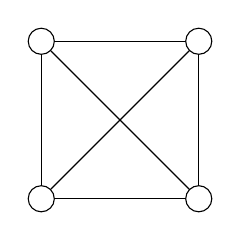
\begin{tikzpicture}
  \node[circle, draw] (A) at (0,0) {};
  \node[circle, draw] (B) at (2,0) {};
  \node[circle, draw] (C) at (2,2) {};
  \node[circle, draw] (D) at (0,2) {};

  \draw (A) -- (B);
  \draw (A) -- (C);
  \draw (A) -- (D);
  \draw (B) -- (C);
  \draw (B) -- (D);
  \draw (C) -- (D);
\end{tikzpicture}
    \end{ex}
\end{graybox}

\begin{bluebox}
    \begin{defn}
    The \textbf{order} of a graph $G$ is $|V(G)|$ and the \textbf{size} of $G$ is $|E(G)|$.
\end{defn}
\end{bluebox}

\begin{bluebox}
    \begin{defn}
    Vertices $u$ and $v$ are \textbf{adjacent} in $G$ if $uv \in E(G)$. The \textbf{endpoints} of the edge $uv$ are $u$ and $v$.
\end{defn}
\end{bluebox}

\begin{bluebox}
    \begin{defn}
    A vertex $v$ is \textbf{incident} to edge $e$ if $v$ is an endpoint of $e$.
\end{defn}
\end{bluebox}

\begin{bluebox}
    \begin{defn}
    The \textbf{(open) neighborhood} of $v\in V(G)$ is
    \[N(v) = \{ u \in V(G) | uv \in E(G) \}\]
\end{defn}
\end{bluebox}
$N(v)$ is the set of all vertices in $G$ that are adjacent to $v$.

\begin{bluebox}
    \begin{defn}
        The \textbf{degree} of a vertex is
        \[\deg(v) = |N(v)|\]
    \end{defn}
\end{bluebox}
$\deg(v)$ is simply the number vertices that are adjacent to $v$. In a general graph, $\deg(v)$ is the number of edges incident to $v$ since loops and parallel edges are also counted.

\begin{bluebox}
    If $\deg(v) = 0$, $v$ is an \textbf{isolated vertex}.
\end{bluebox}

\begin{bluebox}
    The graph $G$ is a \textbf{subgraph} of a graph $H$ $(G \leq H)$ if $V(G) \subseteq V(H)$ and $E(G) \subseteq E(H)$
\end{bluebox}

\begin{graybox}
    \begin{ex}
    The graph on the right is a subgraph of the graph on the left.
    \center
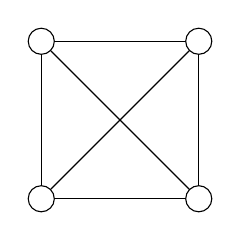
\begin{tikzpicture}
  \node[circle, draw] (A) at (0,0) {};
  \node[circle, draw] (B) at (2,0) {};
  \node[circle, draw] (C) at (2,2) {};
  \node[circle, draw] (D) at (0,2) {};

  \draw (A) -- (B);
  \draw (A) -- (C);
  \draw (A) -- (D);
  \draw (B) -- (C);
  \draw (B) -- (D);
  \draw (C) -- (D);
\end{tikzpicture}
\hspace{32pt}
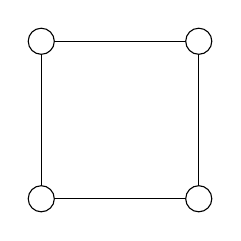
\begin{tikzpicture}
  % Define the 4 unlabeled nodes in a square (cycle)
  \node[circle, draw] (A) at (0,0) {};
  \node[circle, draw] (B) at (2,0) {};
  \node[circle, draw] (C) at (2,2) {};
  \node[circle, draw] (D) at (0,2) {};

  % Draw the cycle edges
  \draw (A) -- (B);
  \draw (B) -- (C);
  \draw (C) -- (D);
  \draw (D) -- (A);
\end{tikzpicture}
    \end{ex}
\end{graybox}

\begin{bluebox}
    \begin{defn}
        A graph $G$ is an \textbf{induced subgraph} of a graph $H$ if $G$ is obtained from $H$ by deleting vertices (every time a vertex is deleted, so are all incident edges).
    \end{defn}
\end{bluebox}

\begin{graybox}
    \begin{ex}
    The graph on the right, $C_3$, is an induced subgraph of the $K_4$ on the left. We get $C_3$ from $K_4$ by removing any vertex (and all of its incident edges).
    \center
    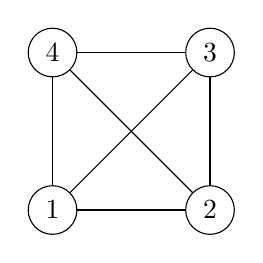
\begin{tikzpicture}
  \node[circle, draw] (A) at (0,0) {1};
  \node[circle, draw] (B) at (2,0) {2};
  \node[circle, draw] (C) at (2,2) {3};
  \node[circle, draw] (D) at (0,2) {4};

  \draw (A) -- (B);
  \draw (A) -- (C);
  \draw (A) -- (D);
  \draw (B) -- (C);
  \draw (B) -- (D);
  \draw (C) -- (D);
\end{tikzpicture}
\hspace{32pt}
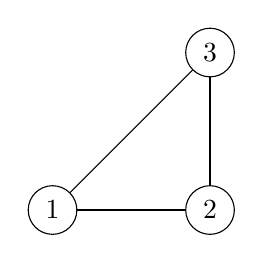
\begin{tikzpicture}
  \node[circle, draw] (A) at (0,0) {1};
  \node[circle, draw] (B) at (2,0) {2};
  \node[circle, draw] (C) at (2,2) {3};

  \draw (A) -- (B);
  \draw (A) -- (C);
  \draw (B) -- (C);
\end{tikzpicture}
    \end{ex}
\end{graybox}

The induced subgraph of $H$ with the set of vertices in $S$ is denoted by $H[S]$.

In Example $2.3$, we would say the induced subgraph is $C_4[\{1,2,3\}]$.

\begin{bluebox}
    \begin{defn}
        $G$ is a \textbf{spanning subgraph} of $H$ if $G$ is obtained from $H$ by only deleting edges.
    \end{defn}
\end{bluebox}

\begin{bluebox}
    \begin{defn}
        If $ G \leq H$, then we say $H$ is a \textbf{supergraph} of $G$.
    \end{defn}
\end{bluebox}

\begin{bluebox}
    \begin{defn}
    The \textbf{length} of a path or cycle is the number of edges.
\end{defn}
\end{bluebox}

\begin{bluebox}
    \begin{defn}
        A graph $G$ is \textbf{connected} if for all $u,v \in V(G)$, there exists a path from $u$ to $v$.
    \end{defn}
\end{bluebox}

When a graph is disconnected, it is comprised of some number of components. These components are themselves connected, but they aren't connected to each other.

\begin{bluebox}
    \begin{defn}
        A \textbf{separating set} $S$ of $G$ is a set of vertices or edges (exclusively) such that $G - S$ has more components than $G$.
    \end{defn}
\end{bluebox}

\begin{bluebox}
    \begin{defn}
        A vertex $v$ is a \textbf{cut-vertex} if $\{v\}$ is a separating set.
    \end{defn}
\end{bluebox}

\begin{bluebox}
    \begin{defn}
        A graph is \textbf{$k-$connected} if there are no vertex separating sets of size less than $k$.
    \end{defn}
\end{bluebox}

Alternatively, we can say a graph is $k-$connected if at least $k$ vertices need to be deleted so that the resulting graph is disconnected.

\begin{figure}[htb!]
  \centering
  \begin{subcaptionbox}{$K_5$\label{fig:fig1}}[0.25\textwidth]
    {\includegraphics[width=\linewidth]{graphs/K_5.png}}
  \end{subcaptionbox}
  \hspace{0.05\textwidth}
  \begin{subcaptionbox}{$K_{3,3}$\label{fig:fig2}}[0.25\textwidth]
    {\includegraphics[width=\linewidth]{graphs/K_3,3.png}}
  \end{subcaptionbox}
  \caption{$k-$subs}
  \label{fig:combined}
\end{figure}

There are two graphs that are particularly important to understanding Kuratowski's Theorem. These are $K_5$ and $K_{3,3}$. $K_{x,y}$ denotes the graph where the we partition the vertex set into $2$ subsets, and we draw edges from one set to another, but not within a set themselves.

\section{A Short Introduction to Planarity}
\begin{bluebox}
    \begin{defn}
        A graph $G$ is \textbf{embeddable} on a surface $S$ if it can be drawn on $S$ so that no two edges intersect (unless they have a common endpoint and intersect at that incident vertex).
    \end{defn}
\end{bluebox}

\begin{bluebox}
    \begin{defn}
        A graph $G$ is \textbf{planar} if it can be embedded in the Euclidean plane.
    \end{defn}
\end{bluebox}

\begin{greenbox}
\begin{lem}(Euler's Formula)
    If a graph $G$, with $v$ vertices and $e$ edges, is planar and has $f$ faces, $v-e + f = 2$.
\end{lem}
\end{greenbox}

\begin{proof}
    Let $T$ be a proper and planar subgraph of $G$ that contains all $v$ vertices and no cycles. $T$ has $v$ vertices, $v - 1$ edges, and $1$ face. So the Lemma is true for $T$. Now, we can add all the edges of $G$ back to $T$ sequentially.

    Note that, whenever an edge is added, there will be a cycle in the graph, and the existing face is broken into two new ones. So, the number of edges added equals the number of new faces.
    So the formula holds for $G$.
\end{proof}

    \noindent Note that any face in a planar graph must be bordered by at least $3$ edges.

\begin{greenbox}
\begin{lem}
    If $G$ is planar with $v$ vertices and $e$ edges, $e \le 3v -6$.
\end{lem}
\end{greenbox}

\begin{proof}
    Suppose there are $G$ has $f$ faces. We can try to find an inequality for the number of faces in terms of $f$. Each face is comprised of at least 3 edges (which gives $3f$ edges), however, if we sum the number of edges over all the faces, each edge is counted exactly twice. Therefore, $e \geq \dfrac{3f}{2}$, or $f \leq \dfrac{2e}{3}$

    Applying into the Euler's Formula, $$2 = v-e+f \le v-e+\frac{2e}{3} = v - \frac{e}{3}$$ Thus, $e \le 3v-6$.
\end{proof}

\begin{greenbox}
\begin{lem}
    Let $G$ be a planar graph with no odd cycles, and $G$ has $f$ faces and $e$ edges. Then $e + 4 \le 2v$.
\end{lem}
\end{greenbox}

\begin{proof}
    Since $G$ has no odd cycles, each face is bordered by at least $4$ edges, and each of those edges will be counted twice. So $2e \geq 4f$.

    Applying to the Euler's formula, $$2 = v-e+f \le v -e+\frac{e}{2} = v-\frac{e}{2}$$ Thus, $e+4 \le 2v$.
\end{proof}

\begin{greenbox}

\begin{prop}
    $K_5$ and $K_{3,3}$ are not planar.
\end{prop}
\end{greenbox}

\begin{proof}

    $K_ 5$ has $5$ vertices and $10$ edges. By Lemma $3.2$, $K_5$ is not planar.

    $K_{3,3}$ contains no odd cycles. $K_{3,3}$ has $6$ vertices and $9$ edge. By Lemma $3.3$, $K_{3,3}$ is not planar.

\end{proof}

\section{Kuratowski's Theorem - Part 1: Lemmas and Important Definitions}
    \begin{bluebox}
        \begin{defn}
            To \textbf{contract }an edge $e = ab \in E(G)$, delete the vertices $a$ and $b$, then add a new vertex $v_c$ that is adjacent to each vertex in $[N(a) \cup N(b)] \setminus \{a,b\}$ (all vertices adjacent to $a$ or $b$).
        \end{defn}
    \end{bluebox}

    \begin{bluebox}
        \begin{defn}
            Let $e \in E(G)$. Then, $G \setminus e$ is the graph obtained from $G$ by contracting $e$.
        \end{defn}
    \end{bluebox}

    \begin{graybox}
        \begin{ex}
        Shown below is $C_3$. The graph on the right is the result of contracting the edge $AB$.
        \center
            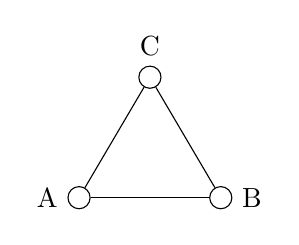
\begin{tikzpicture}[scale=0.9]
                \node[circle, draw, minimum size=8pt, inner sep=0pt, label=left:A] (A) at (0,0) {};
                \node[circle, draw, minimum size=8pt, inner sep=0pt, label=right:B] (B) at (2,0) {};
                \node[circle, draw, minimum size=8pt, inner sep=0pt, label=above:C] (C) at (1,1.7) {};

                \draw (A) -- (B);
                \draw (B) -- (C);
                \draw (C) -- (A);
            \end{tikzpicture}
            \hspace{64pt}
            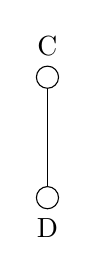
\begin{tikzpicture}[scale=0.9]
                \node[circle, draw, minimum size=8pt, inner sep=0pt, label=below:D] (D) at (1,0) {};
                \node[circle, draw, minimum size=8pt, inner sep=0pt, label=above:C] (C) at (1,1.7) {};

                \draw (D) -- (C);
            \end{tikzpicture}
        \end{ex}
    \end{graybox}

    \begin{bluebox}
        \begin{defn}
            To \textbf{subdivide} an edge $e = ab \in V(G)$, delete $e$ from $E(G)$ and add a new vertex that is adjacent to $a$ and $b$ (exclusively).
        \end{defn}
    \end{bluebox}

    \begin{graybox}
        \begin{ex}
        The edge below is subdivided.
        \begin{center}

    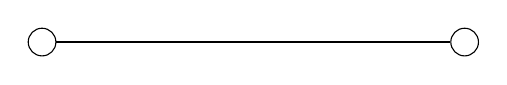
\begin{tikzpicture}[main_node/.style={circle,draw,minimum size=1em,inner sep=3pt]}]

    \node[main_node] (0) at (-4.857142857142858, 4.857142857142858) {};
    \node[main_node] (1) at (0.5095238095238086, 4.857142857142858) {};

    \path[draw, thick]
    (1) edge node {} (0)
    ;
    \end{tikzpicture}


$\Downarrow$
\vspace{10pt}

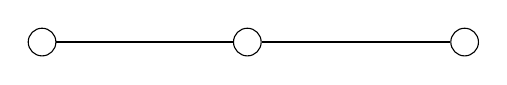
\begin{tikzpicture}[main_node/.style={circle,draw,minimum size=1em,inner sep=3pt]}]

\node[main_node] (0) at (-4.857142857142858, 4.857142857142858) {};
\node[main_node] (1) at (-2.25, 4.857142857142858) {};
\node[main_node] (2) at (0.5095238095238086, 4.857142857142858) {};

 \path[draw, thick]
(1) edge node {} (0)
(2) edge node {} (1)
;

\end{tikzpicture}
        \end{center}
        \end{ex}
    \end{graybox}

    \begin{bluebox}
        \begin{defn}
            A graph $G$ is a \textbf{subdivision} of a graph $H$ if $G$ can be obtained from $H$ by recursively subdividing edges.
        \end{defn}
    \end{bluebox}

    \begin{bluebox}
        \begin{defn}
            The graph $G^{*}$ is obtained from $G$ by subdividing every edge in $E(G)$ exactly once.
        \end{defn}
    \end{bluebox}

    \begin{bluebox}
        \begin{defn}
            A \textbf{Kuratowski subgraph} ($k-$sub) of $G$ is a subgraph of $G$ that is a subdivision of $K_5$ or $K_{3,3}$
        \end{defn}
    \end{bluebox}

    \begin{bluebox}
        \begin{defn}
            The \textbf{branch vertices} of a subdivision $H^{\prime}$ of a graph $H$ are the vertices in $H^{\prime}$ of degree at least 3.
        \end{defn}
    \end{bluebox}
    \noindent Note that for subdivisions of $K_5$ (or $K_{3,3}$), the branch vertices are the vertices that correspond to the vertices in $K_5$ (or $K_{3,3}$). Furthermore, the degrees of the branch vertices in the subdivision are the same as their corresponding degrees in the actual $K_5$ or $K_{3,3}$.

    \noindent Next, we will cover the lemmas that are used in proving Kuratowski's Theorem.

    \textbf{Lemmas}
    \begin{greenbox}
        \begin{lem}
            A graph $G$ is planar if and only if every subdivision of $G$ is planar.
        \end{lem}
    \end{greenbox}

    \begin{greenbox}
        \begin{lem}
            If $G$ is a planar graph, then every subgraph of $G$ is planar.
        \end{lem}
    \end{greenbox}

\section{Kuratowski's Theorem - Part 2: The First Proof}
\begin{greenbox}
    \begin{thrm}[Kuratowski's Theorem]
        A graph $G$ is planar if and only if $G$ does not contain any subgraph that is subdivision of $K_5$ or $K_{3,3}$.
    \end{thrm}
\end{greenbox}

We can state Kuratowski's Theorem more simply. We already know that $K_5$ and $K_{3,3}$ are not planar, so clearly any graph containing one of them as a subgraph is also nonplanar. But we can go further to say that if a graph contains any subgraph that resembles the shape of $K_5$ or $K_{3,3}$ (effectively a subdivision of one of these), then the graph is nonplanar. [2]

Before jumping into the proof, we can discuss the general strategy so that the motivation of some of the steps are clearer. First, this is a proof by minimal counterexample. The general outline for such a proof is shown below.

Here is the overall strategy for proving Kuratowski's Theorem.

\textbf{Strategy for Proof of Kuratowski's Theorem}
\begin{enumerate}
    \item Consider an edge-minimum graph that has no $k-$subs and is nonplanar (this is the minimal counterexample).

    \item Show that the counterexample must be 3-connected.

    \item Show that (2) implies the counterexample is planar, and thus not a counterexample.
\end{enumerate}
Now we're ready to tackle this proof.

\begin{proof}
We can first observe that the forwards direction is very easy to prove. By Lemma $6.1$ and $6.2$. this is obviously true.

We begin the backwards direction with several claims that will be useful when we address the minimal counterexample.
    \begin{greenbox}
        \begin{claim}
            An (edge and vertex)-minimal non-planar graph $G$ is connected.
        \end{claim}
    \end{greenbox}

    \begin{greenbox}
        \begin{claim}
        An (edge and vertex)-minimal non-planar graph $G$ is 2-connected.
        \end{claim}
    \end{greenbox}

    \begin{proof}

        If $G$ is not connected, then $G$ will contain some components. Since every component is also a subgraph, then all of them are planar. Then we can "attach" those components together, one-by-one,  so that the resulting graph is planar, which is a contradiction.

        Suppose $G$ is only $1-$connected, and let $u$ be a cut-vertex. Let $C_i$ be components of $G-u$, then all $C_i \cup \{i\}$ are planar. Then we can "join" all $C_i$ and $u$ together so that the resulting graph is planar, which is a contradiction.

        So $G$ is $2-$connected.

    \end{proof}

    \begin{figure}[hbt!]
        \centering
        \includegraphics[width=0.25\linewidth]{graphs/component_and_v.png}
        \caption{Example $V(C_i) \cup \{v\}$}
    \end{figure}

    \begin{greenbox}
        \begin{claim}
            Suppose $\{x,y\}$ is a 2-separating set of a graph $G$ and $C_1, \ldots, C_k$ are the components of $G - \{x,y\}$. For each $1 \leq i \leq k$, let $G_i^{\prime} = G[V(C_i) \cup \{x,y\}] + xy$. If $G$ is non-planar, then at least one $G_i^{\prime}$ is non-planar.
        \end{claim}
    \end{greenbox}
    \noindent The graphs $G_i^{\prime}$ in this claim are very similar to the induced subgraphs in Claim 2. However, the primary difference is that we're adding the edge $xy$. $xy$ may or may not exist in $G$, but whether or not it does, we know it will be present in each of the $G_i^{\prime}$ graphs.

     \begin{figure}[hbt!]
        \centering
        \includegraphics[width=0.40\linewidth]{graphs/connect_components_and_xy.png}
        \caption{Possible graphs for $G_1^{\prime}, G_2^{\prime}$, and $G_3^{\prime}$}
    \end{figure}
    \noindent Observe that we can identify each of the $G_i^{\prime}$ at $xy$, we get something that is very close the original graph $G$. We get the supergraph $G + xy$. If $xy \in E(G)$, then this simply $G$.

    \begin{proof}
        Suppose that each $G_i^{\prime}$  is planar.
        Our strategy for this proof will be to find some way to glue all of the $G_i^{\prime}$ together so that the result, $G + xy$ is planar.
        Then because $G + xy$ is a supergraph of $G$, $G$ must be planar.
        \begin{figure}
            \centering
            \includegraphics[width=0.25\linewidth]{graphs/embedding_G_xy.png}
            \caption{Our planar embedding of $G + xy$}
        \end{figure}

        Since $xy$ is an edge in $G_1^{\prime}$, it is on the boundary of some face of $G_1^{\prime}$. $G_2^{\prime}$ can be drawn in that face and identify the copies of $xy$. Then, we can draw $G_3^{\prime}$ in a face of this graph and identify it through the edge $xy$. We can continue this process until the last component of $G - \{x,y\}$.

        The resulting graph is $G + xy$ (shown in figure $3$), so we have shown that $G + xy$ is planar, which means $G$ is planar.
    \end{proof}

\begin{greenbox}
    \begin{claim}
        If $H$ is a k-sub free non-planar graph with the fewest possible number of edges, then $H$ has one $3-$connected component and the rest of the components are isolated vertices.
    \end{claim}
\end{greenbox}

\begin{proof}
    The isolated vertices don't affected the connectivity of the one $3$-connected component, so we can delete all of the isolated vertices of $H$ to obtain the subgraph $G$. $G$ is still $k-$sub free and non-planar with the fewest number of edges possible.

    Because $G$ is edge-minimally $k$-sub free and non-planar, deleting an edge must result in a subgraph that is planar. Because $G$ has no isolated vertices, deleting a vertex implies that at least one edge is also deleted. So, deleting vertices also produces a planar subgraph. Therefore, $G$ is (edge and vertex)-minimally non-planar. By Claim 2, $G$ is 2-connected.

    Now, suppose that $\{x,y\}$ is a $2-$separating set of $G$ with components $C_1, \ldots, C_k$ of $G - \{x,y\}$. Since $G$ is non-planar, there exists a $G_i^{\prime}$ (from the definition in Claim 3) that is non-planar by Claim 3. Since $G$ is 2-connected, both $x$ and $y$ must be incident to an edge that goes into a component that is not $C_i$. Otherwise, either $x$ or $y$ would be a cut-vertex, thus contradicting $G$ being 2-connected. That is, if $x$ was the only vertex of $x$ and $y$ that was connected to other components, then deleting $x$ would disconnected the graph, making $x$ a cut vertex.

    \begin{figure}[hbt!]
        \centering
        \includegraphics[width=0.35\linewidth]{graphs/c_i_xy.png}
        \caption{}
    \end{figure}
    \noindent Therefore, $|E(G_i^{\prime})| \leq |E(G)| + 1 - 2 = |E(G)| - 1 < |E(G)|$. We add 1 because in the worst case scenario, $xy$ doesn't exist $G$ while it exists in $G_i^{\prime}$. We add 2 because we concluded that there are at least two edges originating from $x$ and $y$ that go outside of $G_i^{\prime}$, so they wouldn't be included in $|E(G_i^{\prime})|$. We get the inequality because there could be more than $2$ edges incident to $x$ and $y$ outside of $G_i^{\prime}$, and $xy$ might already exist in $G$.

    $G$ is edge-minimally $k-$sub free and non-planar, so $|E(G_i^{\prime})| < |E(G)|$, $G_i^{\prime}$ must either have a k-sub or be planar. However, we already know that $G_i^{\prime}$ is non-planar, so it must be that $G_i^{\prime}$ contains a k-sub.

    Now we have that $G$ has no k-sub but $G_i^{\prime}$ does have a k-sub. The difference is that $G_i^{\prime}$ contains $xy$. So it must be the case that adding $xy$ created the k-sub in $G_i^{\prime}$. This means that $xy$ is not in $G$ and it is in the k-sub in $G_i^{\prime}$.
    \begin{figure}[hbt!]
        \centering
        \includegraphics[width=0.35\linewidth]{graphs/k_sub_xy.png}
        \caption{}
    \end{figure}

    Let $C_j$ be a different component of $G - \{x,y\}$.  Note, both $x$ and $y$ have a neighbor in $C_j$. If only one of them had a neighbor in $C_j$, then that vertex ($x$ or $y$) would be a cut vertex.
    Since $C_j$ is connected, there is an $x-y$ path $P$ in $G$ whose internal vertices are in $C_j$. Therefore, the vertices in the k-sub of $G_i^{\prime}$ and the vertices in $P$ form a subdivision of the k-sub in $G_i^{\prime}$ (see Figure $7$). This is because $P$ acts like the edge $xy$ that created the k-sub mentioned previously.

    Thus, $G$ has a $k-$sub, which is a contradiction. Therefore, $G$ is $3-$connected.

\end{proof}

\begin{figure}[hbt!]
    \centering
    \includegraphics[width=0.50\linewidth]{graphs/k_sub_i_j.png}
    \caption{}
\end{figure}

\begin{greenbox}
    \begin{claim}
        If $G$ has no k-subs and $e \in E(G)$, then $G / e$  has no k-subs.
    \end{claim}
\end{greenbox}

    \begin{proof}
        We're going to prove this claim via contrapositive. This means we're trying to show that if $G/e$ has a $k-$sub, then $G$ has a $k-$sub. Let $e = xy \in E(G)$ such that $G / e$ has a k-sub, call it $H$.
        Let $v_e$ be the new vertex in $G /e$ obtained by contracting $e$.

        \textbf{Case 1: }First, if $v_e \not \in V(H)$, then $H$ is a subgraph of $G$ and we're done since $G$ already had a k-sub before contracting $e$.

        \textbf{Case 2:} If $v_e \in V(H)$ but $v_e$ is not a branch vertex of $H$, then we can find a subdivision of $H$ in $G$ by replacing $v_e$ in $H$ with either $x$, $y$, or the edge $xy$. Note that by replacing $v_e$ with $xy$ (thereby undoing the contraction) creates a copy of $H$ or a subdivision of $H$. We're trying to track what happens when we undo the contraction because we want to get back to $G$ and show that it has a k-sub. Then, we're tracking the three different cases for how we could undo the contraction.
        \begin{figure}[hbt!]
            \centering
            \includegraphics[width=0.6\linewidth]{graphs/pre_contraction.png}
            \caption{The three possible configurations in $G$ before the contraction}
        \end{figure}

        In Figure $8$, the path on the left (containing $v_e$) is in $G/e$, while the graphs on the right are in $G$. Notice that the path containing $v_e$ still exists in each of possible pre-contraction subgraphs in $G$. Because $v_e \in V(H)$, $G$ also contains a k-sub.

        \textbf{Case 3:} Suppose $v_e \in V(H)$ is a branch vertex of $H$ and one of $x$ or $y$ (say $x$) contributes (recall that when we contract $e = xy$, we take the union of the neighborhoods of $x$ and $y$ to get the vertices adjacent to $v_e$) at most one edge to $\deg_H(v_e)$. Then we can obtain a k-sub in $G$ from $H$ where $y$ is the new branch vertex and $x$ subdivides an edge incident to $y$.
        \begin{figure}[hbt!]
            \centering
            \includegraphics[width=0.5\linewidth]{graphs/contribute_contraction.png}
            \caption{}
        \end{figure}

        Figure $9$ shows how in $G$ we have that $x$ contributes 1 to $\deg_H(v_e)$. We also see $v_e$'s place in the subdivision $H$. However, notice that if move around $x$ in $G$, we have the same setup as in $H$ except $x$ subdivides the top edge.

        Therefore, the k-sub also exists in $G$.

        Note, that Case 3 covers the situation in which $H$ is a subdivision of $K_{3,3}$. This is because every vertex in $K_{3,3}$ has degree 3, which means $\deg_H(v_e)$ is 3. That is, because $\deg_H(v_e) \leq 3$, it must be one of the vertices that correspond to actual an actual vertex in $K_{3,3}$ or $K_5$. Vertices that arise from subdivisions have degree 2. Therefore, the only cases we could have for how $x$ and $y$ contribute to $\deg_H(v_e)$ are (1) $x$ contributes 0 and $y$ contributes 3, (2) $x$ contributes 1 and $y$ contributes $2$, (3) $x$ contributes $2$ and $y$ contributes $1$, and (3) $x$ contributes 3 and $y$ contributes 0. In each case, one of $x$ or $y$ contributes at most $1$ to the degree.

        \textbf{Case 4:} If $H$ is a subdivision of $K_5$ and $v_e$ is a branch vertex where $x$ and $y$ each contribute exactly 2 (this avoids crossing with Case 3). Observe that we specify $K_5$ because of the observation at the end of Case 3.

        So, $x$ contributes 2 "neighbors" of $v_e$ in the subdivision of $K_5$ in $G/e$. Let $u_1$ and $u_2$ be the branch vertices in $H$ that correspond to those "neighbors" of $v_e$. Let $v_1$ and $v_2$ be the same for $y$.
        \begin{figure}[hbt!]
            \centering
            \includegraphics[width=0.8\linewidth]{graphs/uncontracted.png}
            \caption{}
        \end{figure}

        In this case, we find a subdivision of $K_{3,3}$ in $G$ from $H$ by uncontracting $v_e$ and deleting the $u_1u_2$ path and the $v_1v_2$ path in $H$. This gives the subdivision of $K_{3,3}$ shown in Figure 11.
        \begin{figure}[hbt!]
            \centering
            \includegraphics[width=0.25\linewidth]{graphs/subdivision_K_3,3_1.png}
            \caption{}
        \end{figure}

        Therefore, $G$ contains a subdivision.

        \end{proof}

        \begin{greenbox}
            \begin{claim}
                If $|G| \geq 5$ and $G$ is 3-connected, there exists an edge $e \in E(G)$ such that $G/e$ is 3-connected.
            \end{claim}
        \end{greenbox}
        \begin{proof}
            Suppose there is a $2$-separating set $S$ of $G/e$ where $e = xy \in E(G)$. Since $G$ is 3-connected, the vertex $v_e$ obtained by contracting $e$ must be in $S$.
            Otherwise, $S$ includes two vertices that are not $x$ or $y$, which means $S$ is also a separating set in $G$ and $G$ is not 3-connected.
            Let $z$ be the other vertex in $S$ and say $z$ is the "mate" of the pair $x,y$. Note, $G - \{x,y,z\}$ is disconnected.

            Suppose that no edge $e \in E(G)$ can be contracted such that $G / e$ is 3-connected. Thus, every edge $xy \in E(G)$ has a "mate" $z$. Choose $e = xy$ and its mate $z$ such that the largest number of vertices in any component of $G - \{x,y,z\}$ is maximum. Let $H$ be this largest component and let $H^{\prime}$ be any other component of $G - \{x,y,z\}$. Since $G$ is 3-connected, each of $x,y$, and $z$ have both a neighbor in $H$ and in $H^{\prime}$.
            \begin{figure}[hbt!]
                \centering
                \includegraphics[width=0.40\linewidth]{graphs/claim_6.png}
                \caption{}
            \end{figure}

            Figure 12 shows what happens if $x$ and $z$ have neighbors in both $H$ and $H^{\prime}$ while $y$ has a neighbor in only one of the components. In this case, $\{x,z\}$ is a 2-separating set, which contradicts $G$ being 3-connected. We would get similar diagrams for when $x$ or $y$ are connected to only one of the components.

            Let $u$ be a neighbor of $z$ in $H^{\prime}$ and let $v$ be a mate of $zu$, which we know exists by a previous assumption. Note that $v \not \in \{x,y\}$. This is because if we deleted $zu$ and $x$, the components would still be connected via the path from $H$ to $H^{\prime}$ containing $y$. Similar reasoning shows $v \not  = y$.

            If $v \in H$, then deleting $v$ disconnects $G[V(H) \cup \{x,y\}]$. This is because after deleting $z$ and $u$, $v$ must be responsible for completing the disconnection of $H$ and $H^{\prime}$. Therefore it must disconnect the induced subgraph. In this case, $G - \{v,z\}$ is disconnected. These two do the job without $u$, which is a contradiction since $G$ is 3-connected.

            Thus, $v \in H^{\prime}$. However, this means that $G[V(H) \cup \{x,y\}]$ is contained in a component of $G - \{z,u,v\}$ that is larger than $H$, $\rightarrow \leftarrow$. Thus, there exists an edge $e \in E(G)$ such that $G / e$ is 3-connected.
    \end{proof}

    \begin{greenbox}
        \begin{claim}
            If $G$ is 3-connected with no k-subs, then $G$ is planar.
        \end{claim}
    \end{greenbox}

    \begin{proof}
        We will proceed by induction on the number of vertices.

        \textbf{Base: }If $|G| \leq 4$ (we do this because Claim 6 works for $|G| \geq 5$) and $G$ is 3-connected, then $G \cong K_4$, which is planar.

        \textbf{Inductive: }Suppose every 3-connected k-sub free graph on at most $q$ vertices is planar (for a  fixed $q \geq 4$).

        Let $G$ be a 3-connected k-sub free graph on $q + 1$ vertices. By Claim 6, let $e = xy \in E(G)$ such that $G / e$ is 3-connected. By Claim 5, $G /e$ has no k-subs. By the induction hypothesis, $G / e$ is planar.

        Let $v_e$ be the vertex obtained by contracting $e$. Let $E(v_e)$ be the set of vertices adjacent to $v_e$. Note, $H = G/e - E(v_e)$ is also planar since we're just deleting edges from a planar graph. Additionally, $v_e$ is an isolated vertex in some face $f$ of $H$ since we've deleted all the edges incident to $v_e$. Since $G / e$ is 3-connected, $G / e - v_e$ is 2-connected. This is because if $G / e - v_e$ had a cut-vertex (making it not 2-connected), then $G / e$ would have a 2-separating set, the cut vertex and $v_e$.

        Note that the boundary of every face of a 2-connected graph plane graph is a cycle (if a boundary of a face isn't a cycle, then we have a cut-vertex). Thus, we can draw $H$ so that $f$ is bounded (and the boundary of $f$ is a cycle).

        Because we deleted all of the edges incident to $v_e$, we deleted all the neighbors of $x$ or $y$. Now that we put $v_e$ inside $f$, it must be that all the neighbors of $x$ and $y$ attach to the cycle. Let $x_0, x_1, \ldots, x_{k-1}$ be the neighbors of $x$ in $G$  in cyclic order clockwise around boundary of $f$.

        \textbf{Case 1: }If $N_G(y) \backslash \{x\}$ is contained inclusively between some $x_i$ and $x_{i+1} (\hspace{-8pt}\mod k)$ around the cycle, then we can draw $y$ in that wedge to see that $G$ is planar.
        \begin{figure}[hbt!]
            \centering
            \includegraphics[width=0.3\linewidth]{graphs/claim_7_1.png}
            \caption{Case 1}
        \end{figure}

        \textbf{Case 2:} If $y$ has a neighbor $u$ strictly inside some wedge from $x_i$ to $x_{i+1}$ and a neighbor $v$ strictly outside that wedge, then $G$ contains a subdivided $K_{3,3}$, which is a contradiction since $G$ contains no k-subs. To see this, consider the vertices $x_i, x_{i+1}, u, v, x$, and $y$ in Figure 14. The vertices $x_i, x_{i+1}, y$ represent one part of $K_{3,3}$ and the remaining vertices represent the other part, so this set of 6 vertices are the branch vertices of the k-sub of $K_{3,3}$.
        \begin{figure}[hbt!]
            \centering
            \includegraphics[width=0.3\linewidth]{graphs/claim_7_2.png}
            \caption{Case 2}
        \end{figure}

        Before addressing Case 3, not that if $x$ and $y$ have at most 2 neighbors in common in the cycle, then we are covered by either Case 1 or Case 2 (we might be have to switch the roles of $x$ and $y$ to see this).

        \textbf{Case 3:} If $x$ and $y$ have 3 common neighbors on the cycle, then $G$ contains a subdivided $K_5$. Each of the 5 vertices in Figure 15 have degree 4.

        \begin{figure}[hbt!]
            \centering
            \includegraphics[width=0.3\linewidth]{graphs/claim_7_3.png}
            \caption{Case 3}
        \end{figure}

        Note that in each case, there could be (and likely are) more vertices on the cycle; that is why we get subdivisions.

        Because Case 2 and Case 3 produce contradictions, we must have Case 1. Therefore, $G$ is planar.
    \end{proof}
    Now we are ready to finish the proof. Recall that our goal is to prove that if $G$ has no k-subs, then $G$ is planar.

    Suppose there is a counterexample, a graph that has no k-subs and is planar. Let $G$ be an edge-minimum non-planar k-sub free graph. By Claim 4, $G$ is 3-connected (with possibly isolated vertices). By Claim 7, $G$ is planar.
\end{proof}

\noindent We found this proof in Dr. Joshua Carlson's 3-part video series [1] on Kuratowski's Theorem. Most of the explanations included in the text above come from Joshua Carlson.

\begin{section}{Kuratowski's Theorem - Part 3: The Other Proof}

In this section, we present another proof of this theorem. The set-up is mostly the same, but a different approach is covered.

\textbf{Proof by Minimal Counterexample}

\begin{enumerate}
    \item Consider a minimal counterexample
    \item Prove that this counterexample must contain a subgraph that is subdivision of $K_5$ or $K_{3,3}$
\end{enumerate}


\textbf{Strategy}
In this proof, we will use some results from earlier proof. Particularly, we will use the following:

\begin{enumerate}
    \item Suppose $G$ is an edge-minimum graph that has no $k-$subs and is nonplanar
    \item $G$ is $2-$connected
    \item $G$ has one edge that, when removed, will stay $2-$connected
\end{enumerate}

We also introduce a new lemma.

\begin{greenbox}
\begin{lem}
If $G$ is $2-$connected, then for every pair of $u,v \in V(G)$, there exists a cycle, composes of two internally-disjoint paths, that includes both $u$ and $v$.
\end{lem}
\end{greenbox}

\begin{proof}
We will prove this by induction on the distance of $u$ and $v$.

\textbf{Base:} Suppose $d(u, v) = 1$, then $uv$ is an edge. If $deg(v) = 1$, then $u$ is a cut-vertex. Let $w$ be a neighbor of $v$. Now temporarily remove $v$. Since $G$ is $2-$connected, $G- v$ is connected, and there exists a path in $G-v$ that connects $u$ and $w$. Adding back $v$ into $G$, then the subgraph constructed by that path, edge $vw$, and edge $uv$ is a cycle that contains both $u$ and $v$.

\textbf{Inductive:} Suppose this holds true if $1 \le d(u,v) \le d-1$.

Suppose there exists two vertices $u,v$ in $G$ such that $d(u,v) = d$ along a path $Q$. Let $w$ be a neighbor of $v$ in $Q$. Then by induction hypothesis, there exists a cycle $C$ that contains both $u$ and $w$. If $v$ is on $C$, then we are done. If $v$ is not on $C$, since $G$ is $2-$connected, then there exists a path connecting $u$ and $v$ in $G-w$. We then "trace the outline" to form a cycle between $u$ and $v$.
\end{proof}

\begin{figure}[hbt!]
    \centering
    \includegraphics[width=0.5\linewidth]{graphs/trace_outline.png}
    \caption{Tracing the outline}
\end{figure}

\noindent Now we can start the proof.

\begin{proof}

Let $G$ be a nonplanar graph such that any proper subgraph of $G$ is planar. Suppose that $G$ does not has no $k-$subs.

From Claim $3$ above, suppose $G$ has an edge $uv$ such that $ H = G \setminus\{uv\}$ is $2-$connected. Since $H$ is $2-$connected, by Lemma $6.1$, there exists a cycle in $H$ that contains both $u$ and $v$.

Among all embeddings of $H$, let $C$ be such cycle such that the number of regions inside $C$ is maximized. We denote $C$ as the closed path $u = v_0, v_1, \dots, v = v_n, v_{n+1}, \dots, v_\ell, v_0$.

We observe the following:
\begin{enumerate}
\item There is no path between any vertices of $\{ v_0, v_1, \dots, v_n \}$.
\item There is no path between any vertices of $\{ v_n, v_{n+1}, \dots, v_0\}$.
\end{enumerate}

\begin{proof}
  If there is any such path, we can "trace the outline" of that path and $C$ to obtain a larger cycle, which is a contradiction.
\end{proof}

\begin{figure}
    \centering
    \includegraphics[width=0.4\linewidth]{graphs/set_up.png}
    \caption{The set-up}
\end{figure}

Note that, $H$ is planar, and $G$ is nonplanar, so there must be some "structures" in and around $C$ that prohibit us from adding the edge $uv$.

For the exterior structures, there must be a path, $P$, lying to the outside of $C$ that connects some vertex in $\{v_0, v_1, \dots, v_{n-1} \}$ and some vertex in $\{ v_{n+1}, v_{n+2}, \dots, v_{\ell} \}$. Let $v_k, v_j$ be the endpoints of $P$ that are on $C$.

For the interior structures, there must be some graphs that will prevent us from drawing both the edge $uv$ and the path $P$ in the inside of $C$. Let $w$ be a vertex interior to $C$. Let $A = \{ u, v, v_k, v_j \}$. Then the members of $A$ divide $C$ into $4$ smaller paths, excluding the member of $A$, denotes $i, ii, iii, iv$, counting clockwise, with $i$ be the path between $u$ and $v_k$.

For the following section, two points are connected if there exists a path between them that intersect with $C$ at only the endpoints.

There are only $5$ following cases to consider:
\begin{enumerate}
  \item $w$ is not connected to any members of $A$
  \item $w$ is connected to $1$ member of $A$
  \item $w$ is connected to $2$ members of $A$
  \item $w$ is connected to $3$ members of $A$
  \item $w$ is connected to all members of $A$
\end{enumerate}

\textbf{Case 1:} $w$ must be connected to some vertices in $C$. To prevent from drawing edge $uv$, the path that contains $w$ must be from $i$ or $ii$ to some vertex in $iii$ or $iv$. To prevent drawing the path $P$, that interior path must be from $i$ to $iii$ or $ii$ to $iv$.

\begin{figure}[hbt!]
    \centering
    \includegraphics[width=0.7\linewidth]{graphs/case_1.png}
    \caption{Case 1 (contracting $w$ to the top left vertex)}
\end{figure}

\textbf{Case 2:} WLOG $w$ is connected to $v_k$. To prevent from drawing edge $uv$, $w$ must be connected to some vertex in $iii$ or $iv$. To prevent from drawing the path $P$, $w$ must also connected to another distinct vertex that is in another region among $iii$ and $iv$.

Similar arguments can be made when $w$ is connected to another member of $A$.

\begin{figure}[hbt!]
    \centering
    \includegraphics[width=0.7\linewidth]{graphs/case_2.png}
    \caption{Case 2 (contracting the edge $uv_j)$}
\end{figure}

\textbf{Case 3:} For the example above, if $w$ is connected to $u$, $w$ will connected to a vertex in $iii$. If $w$ is connected to $v$, $w$ is connected to a vertex in $iv$. If $w$ is connected to $v_j$, then the path interior to $C$ containing $w$ will be the path $P$, and we can draw $uv$ in the outside.

\textbf{Case 4:} WLOG $w$ is connected to $u, v$, and $v_j$. To prevent from drawing the edge $uv$, there must be a path connecting from a vertex in the path $uw$ or $vw$ to $v_k$. This graph also prevents from drawing the edge $uv$.

\begin{figure}[hbt!]
    \centering
    \includegraphics[width=0.5\linewidth]{graphs/case_4.png}
    \caption{Case 4}
\end{figure}

\textbf{Case 5:} It is already true.

\begin{figure}[hbt!]
    \centering
    \includegraphics[width=0.3\linewidth]{graphs/case_5.png}
    \caption{Case 5}
\end{figure}

\noindent For the final step, when adding the edge $uv$ back into all $5$ cases to obtain $G$, all of them contain a $k-$sub, which is a contradiction.

\end{proof}

\end{section}

\section{Future Work}

If we had more time, there are several avenues we would pursue. In particular, we would examine a closely related result: Wagner's Theorem. It takes a different approach in characterizing the Kuratowski subgraphs by utilizing minors instead of subdivisions. We would compare the methods used in the proof of Wagner's Theorem with the techniques we encountered in the proofs of Kuratowski's theorem.
\begin{bluebox}
        \begin{defn}
            Suppose $G$ and $H$ are graphs and $H$ can be obtained from $G$ by deleting vertices, deleting edges, and/or contracting edges. Then $H$ is a \textbf{minor} of $G$.
        \end{defn}
    \end{bluebox}

\begin{greenbox}
    \begin{thrm}[Wagner's Theorem]
        A graph $G$ is planar if and only if it does not contain $K_5$ or $K_{3,3}$ as minors.
    \end{thrm}
\end{greenbox}

Additionally, we would investigate any theorems concerning embedding graphs in higher order genera.

We theorize that $K_5$ and $K_{3,3}$ are no longer forbidden subgraphs, but what graph structures are forbidden? We would put most of our effort into investigating genus $1$, but still see if we could make generalizations for all general graph.

While this project is expository, our future work would be more exploratory. It would be interesting to discover which graphs can't be embedded in a torus and attempt to find a list of minimal forbidden subgraphs (like $K_5$ and $K_{3,3}$ in the plane). We would have to decide whether to use subdivisions or minors to interpret our results.

We would also provide a detailed comparison between the two proofs we presented. We commented on some the lemmas from the first proof that would be used in the second proof, however, it would be beneficial to include a more thorough analysis. How are the underlying approaches similar? Could we use reasoning from one proof to make the other proof more efficient?



\begin{thebibliography}{100}
\bibitem{label1}
{Carlson, J. (2021). Kurtowski's Theorem Video Lecture Series}
\bibitem{label2} \href{https://www.math.cmu.edu/~mradclif/teaching/228F16/Kuratowski.pdf}{Ratcliffe, M. (2016). Kuratowski’s Theorem.}


\end{thebibliography}

\end{document}
